\documentclass[25pt,a1paper,landscape]{tikzposter}

%% Tikzposter is highly customizable: please see
%% https://bitbucket.org/surmann/tikzposter/downloads/styleguide.pdf

%% Available themes: see also
%% https://bitbucket.org/surmann/tikzposter/downloads/themes.pdf
\usetheme{Default}
% \usetheme{Rays}
% \usetheme{Basic}
%\usetheme{Simple}
% \usetheme{Envelope}
% \usetheme{Wave}
% \usetheme{Board}
% \usetheme{Autumn}
% \usetheme{Desert}


%% Further changes to the title etc is possible
% \usetitlestyle{Default}
% \usetitlestyle{Basic}
% \usetitlestyle{Empty}
% \usetitlestyle{Filled}
% \usetitlestyle{Envelope}
% \usetitlestyle{Wave}
% \usetitlestyle{verticalShading}
\newcommand*{\articles} 
{
A\_180\_MHz\_0.8\_mu\_m\_BiCMOS\_modular\_memory\_family\_of\_DRAM\_and\_multiport\_SRAM-page1.pdf,
A\_200\_Mhz\_0.8-spl\_mu-m\_BiCMOS\_Modular\_Memory\_Family\_Of\_DRAM\_And\_Multiport\_SRAM-page1.pdf,
A\_5\_Gb-s\_9-port\_application\_specific\_SRAM\_with\_built-in\_self\_test-page1.pdf,
A\_BIST\_algorithm\_for\_bit-group\_write\_enable\_faults\_in\_SRAMs-page1.pdf,
A\_high\_speed\_embedded\_cache\_design\_with\_non-intrusive\_BIST-page1.pdf,
A\_new\_hardware\_fault\_insertion\_scheme\_for\_system\_diagnostics\_verification-page1.pdf,
A\_new\_procedure\_for\_weighted\_random\_built-in\_self-test-page1.pdf,
A\_scan-based\_BIST\_technique\_using\_pair-wise\_compare\_of\_identical\_components-page1.pdf,
A\_serial\_interfacing\_technique\_for\_built-in\_and\_external\_testing\_of\_embedded\_memories-page1.pdf,
Adapting\_an\_industrial\_memory\_BIST\_solution\_for\_testing\_CAMs-page1.pdf,
An\_embedded\_technique\_for\_at-speed\_interconnect\_testing-page1.pdf,
BIST\_of\_PCB\_interconnects\_using\_boundary\_scan\_architecture-page1.pdf,
Built-in\_self-test\_assuring\_system\_integrity-page1.pdf,
Combining\_Built-In\_Redundancy\_Analysis\_with\_ECC\_for\_Memory\_Testing-page1.pdf,
Complete-\_contactless\_I-O\_testing\_reaching\_the\_boundary\_in\_minimizing\_digital\_IC\_testing\_cost-page1.pdf,
Configurable\_BISR\_Chain\_For\_Fast\_Repair\_Data\_Loading-page1.pdf,
Implementing\_Design-for-Test\_within\_a\_Tile-Based\_Design\_Methodology\_-\_Challenges\_and\_Solutions-page1.pdf,
Improved\_Core\_Isolation\_and\_Access\_for\_Hierarchical\_Embedded\_Test-page1.pdf,
Low-Power\_Programmable\_PRPG\_With\_Test\_Compression\_Capabilities-page1.pdf,
MBIST\_Support\_for\_Reliable\_eMRAM\_Sensing-page1.pdf,
MBIST\_Supported\_Multi\_Step\_Trim\_for\_Reliable\_eMRAM\_Sensing-page1.pdf,
Memory\_repair\_logic\_sharing\_techniques\_and\_their\_impact\_on\_yield-page1.pdf,
OCI\_Open\_Compression\_Interface-page1.pdf,
Power-Aware\_At-Speed\_Scan\_Test\_Methodology\_for\_Circuits\_with\_Synchronous\_Clocks-page1.pdf,
Power\_Aware\_Embedded\_Test-page1.pdf,
Reducing\_Test\_Point\_Area\_for\_BIST\_through\_Greater\_Use\_of\_Functional\_Flip-Flops\_to\_Drive\_Control\_Points-page1.pdf,
ScanBist\_A\_Multi-frequency\_Scan-Based\_BIST\_Method-page1.pdf,
ScanBist\_a\_multifrequency\_scan-based\_BIST\_method-page1.pdf,
Scan\_testing\_of\_latch\_arrays-page1.pdf,
Serial\_interfacing\_for\_embedded-memory\_testing-page1.pdf,
Structural\_test\_with\_functional\_characteristics-page1.pdf,
Test\_Point\_Insertion\_with\_Control\_Points\_Driven\_by\_Existing\_Functional\_Flip-Flops-page1.pdf,
Test\_generator\_with\_preselected\_toggling\_for\_low\_power\_built-in\_self-test-page1.pdf,
Test\_point\_insertion\_using\_functional\_flip-flops\_to\_drive\_control\_points-page1.pdf,
Testability\_analysis\_and\_test-point\_insertion\_in\_RTL\_VHDL\_specifications\_for\_scan-based\_BIST-page1.pdf,
Transitioning\_eMRAM\_from\_Pilot\_Project\_to\_Volume\_Production-page1.pdf,
}

\newcommand*{\patentsa} {
1990_11_06_4969148-page1.pdf,
1991_02_26_4996691-page1.pdf,
1994_06_21_5323400-page1.pdf,
1994_09_20_5349587-page1.pdf,
1998_09_22_5812469-page1.pdf,
1999_05_09_5900753-page1.pdf,
1999_07_13_5923676-page1.pdf,
1999_12_07_6000051-page1.pdf,
2000_04_04_6046946-page1.pdf,
2000_09_05_6115827-page1.pdf,
2000_11_07_6145105-page1.pdf,
2001_12_04_6327684-page1.pdf,
2001_12_11_6330681-page1.pdf,
2002_03_26_6363520-page1.pdf,
2002_08_27_6442722-page1.pdf,
2002_09_24_6457161-page1.pdf,
2002_10_03_20020143515-page1.pdf,
2002_10_10_20020147951-page1.pdf,
2002_11_26_6487688-page1.pdf,
2002_12_05_20020184562-page1.pdf
}
\newcommand*{\patentsb} {
2003_01_21_6510534-page1.pdf,
2003_03_18_6536008-page1.pdf,
2003_06_12_20030110457-page1.pdf,
2003_06_19_20030115522-page1.pdf,
2003_08_07_20030146777-page1.pdf,
2003_09_02_6614263-page1.pdf,
2003_09_02_6615392-page1.pdf,
2003_11_13_20030212524-page1.pdf,
2003_11_20_20030217315-page1.pdf,
2003_12_04_20030226073-page1.pdf,
2003_12_11_20030229833-page1.pdf,
2003_12_30_6671839-page1.pdf,
2004_01_01_20040003329-page1.pdf,
2004_05_18_6738938-page1.pdf,
2004_05_20_20040098648-page1.pdf,
2004_06_24_20040123203-page1.pdf,
2004_08_19_20040163015-page1.pdf,
2004_08_19_20040163021-page1.pdf,
2004_12_23_20040257901-page1.pdf,
2005_02_03_20050028059-page1.pdf
}
\newcommand*{\patentsc} {
2005_03_03_20050047229-page1.pdf,
2005_10_27_20050240790-page1.pdf,
2005_10_27_20050240847-page1.pdf,
2005_10_27_20050240848-page1.pdf,
2005_12_08_20050273683-page1.pdf,
2007_11_15_20070266278-page1.pdf,
2008_03_13_20080065929-page1.pdf,
2010_02_11_20100037109-page1.pdf,
2012_04_02_20120198294-page1.pdf,
2012_10_25_20120272110-page1.pdf,
2021_06_10_20210174892-page1.pdf,
2022_07_07_20220215896-page1.pdf,
2022_08_30_11430537-page1.pdf,
2022_11_08_11495315-page1.pdf,
2023_04_13_20230110161-page1.pdf,
2023_06_08_20230178172-page1.pdf,
2023_10_17_11789487-page1.pdf,
2024_01_11_20240013846-page1.pdf,
2024_03_12_11929136-page1.pdf,
2024_03_14_20240087665-page1.pdf
}
\newcommand*{\patentsd} {
2024_04_16_11961576-page1.pdf,
2024_07_23_12046315-page1.pdf,
6745359-page1.pdf,
6760874-page1.pdf,
6763489-page1.pdf,
6829730-page1.pdf,
6862717-page1.pdf,
6868532-page1.pdf,
7139946-page1.pdf,
7155651-page1.pdf,
7188274-page1.pdf,
7191374-page1.pdf,
7194669-page1.pdf,
7219282-page1.pdf,
7257733-page1.pdf,
7370251-page1.pdf,
7424656-page1.pdf,
7617425-page1.pdf,
7757135-page1.pdf,
8516317-page1.pdf,
8683280-page1.pdf
}

\colorlet{backgroundcolor}{white}
\usepackage{fontspec}
\usepackage{graphicx}
\usepackage{pdfpages}
\usepackage{subfigure}
\usepackage{mychronology}
\usepackage{adjustbox}
\setmainfont{FreeSerif}
\setsansfont{FreeSans}

\title{Benoit Nadeau-Dostie}
%\author{1994 - 2024}
%% Optional title graphic
\titlegraphic{
	
\includegraphics[height=4cm]{images/UdeS2.jpg},
	
\includegraphics[height=4cm]{images/LogicVisionLogo3.jpg},
	
\includegraphics[height=4cm]{images/MGC Logo2.jpg},
	
\includegraphics[height=4cm]{images/Siemens2.png}
}
%% Uncomment to switch off tikzposter footer
% \tikzposterlatexaffectionproofoff

\settitle{ \centering \vbox{
%		\@titlegraphic \\[\TP@titlegraphictotitledistance] \centering
		\color{titlefgcolor} {\bfseries \Huge \sc \@title \par}
}}
\def \blw{1}
\tikzset{%
	,chronevent/.style={fill=black,draw=none,opacity=0.5}
	,chronlabel/.style={opacity=1}
	,chrontickslabel/.style={chronlabel}
	,chroneventlabel/.style={chronlabel}
	,eventlabel/.style={chroneventlabel,anchor=south west,yshift=.2\unit,rotate=0}
	,flippedeventlabel/.style={chroneventlabel,anchor=north west,yshift=-.2\unit,rotate=0}
	,eventlabelbottom/.style={chroneventlabel,anchor=south west,yshift=-1cm,rotate=0}     % Bottom label
}

\begin{document}
	
	%\tikz[remember picture,overlay] \node[opacity=0.3,inner sep=0pt] at (current page.center){
\includegraphics[width=\paperwidth,height=\paperheight]{images/PP_CHIP.png}};
	
	\maketitle   
    \end
 
	
	\block[linewidth=\blw]{}{
 		\begin{chronology}[2]{1984}{2024}{\linewidth}
		\event[1984]{1986}{
\includegraphics[height=2cm]{images/UdeS2.jpg}}
		\event[1986]{1994}{
\includegraphics[height=2cm]{images/ntlogo.pdf}}
		\event[1994]{2009}{
%			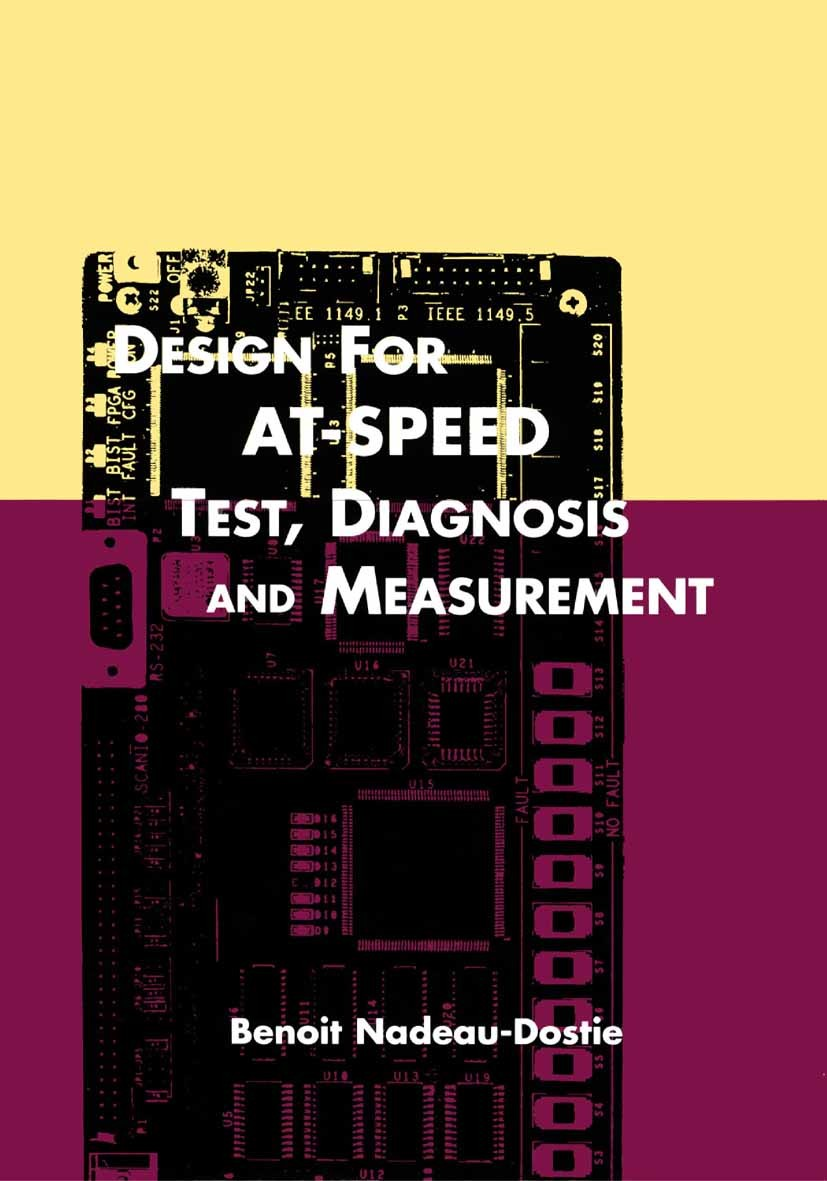
\includegraphics[height=4cm]{images/BND_Book.jpg}
			
\includegraphics[height=2cm]{images/LogicVisionLogo3.jpg},
			}
		\eventpoint{1999}{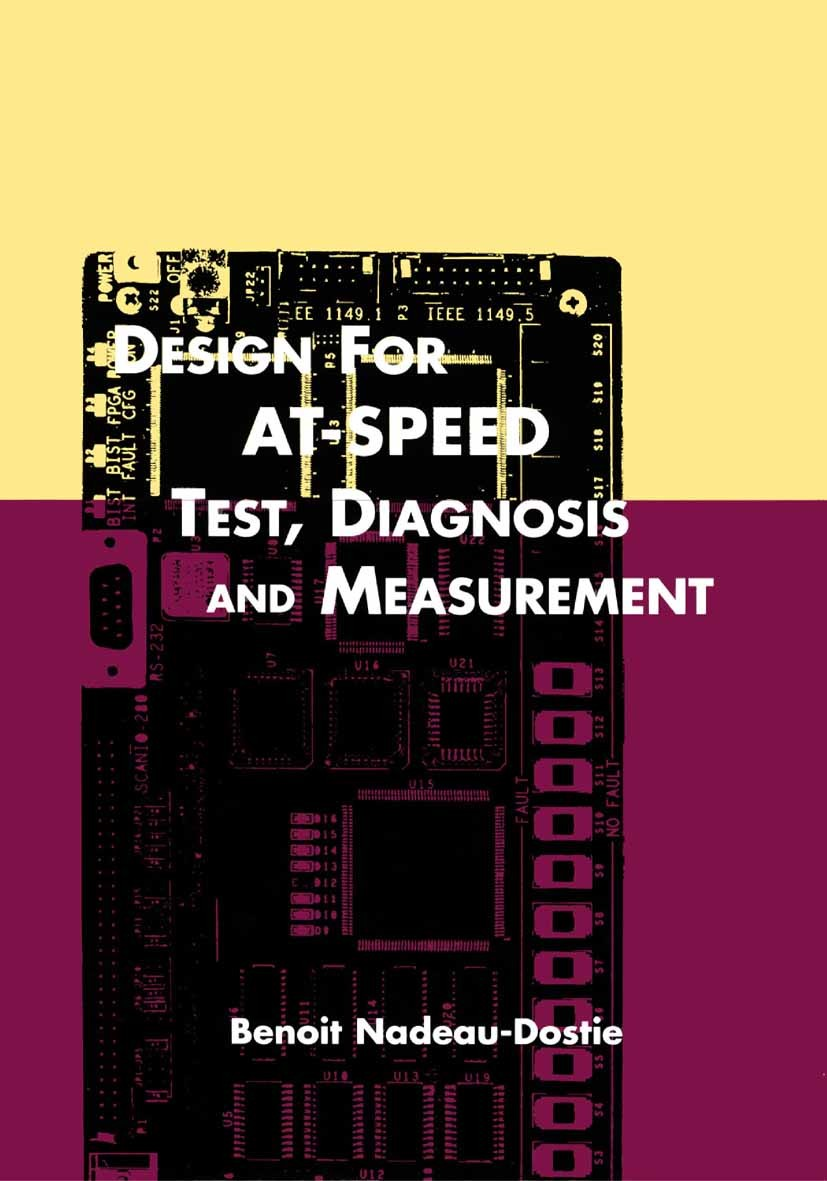
\includegraphics[height=4cm]{images/BND_Book.jpg}}
		\event[2009]{2017}{
\includegraphics[height=2cm]{images/MGC Logo2.jpg}}
		\event[2017]{2024}{
\includegraphics[height=2cm]{images/Siemens2.png}}
		\end{chronology}}
	
    %	\begin{tikzpicture}
	%	% draw horizontal line   
	%	\draw[ultra thick, ->] (0,0) -- (\linewidth,0);
	%	\foreach \x in {0,5,10,15,20,25,30,35,40,45,50,55,60,65,70,75}
	%	\draw (\x cm,3pt) -- (\x cm,-3pt);
	%	\draw[ultra thick] (5,0) node[below=3pt,thick] {1985} node[above=3pt] {};
	%	\draw[ultra thick] (10,0) node[below=3pt,thick] {1990} node[above=3pt] {};
	%	\draw[ultra thick] (15,0) node[below=3pt,thick] {1995} node[above=3pt] {};
	%	\draw[ultra thick] (20,0) node[below=3pt,thick] {2000} node[above=3pt] {};
	%	\draw[ultra thick] (25,0) node[below=3pt,thick] {2005} node[above=3pt] {};
	%	\draw[ultra thick] (30,0) node[below=3pt,thick] {2010} node[above=3pt] {};		
			
	%	\draw[fill=black,draw=none,opacity=0.5,rounded corners=10](10,-0.5) rectangle (20,0.5)%
	%	\draw (10,2) node{
\includegraphics[height=2cm]{images/UdeS2.jpg}}


	%	\end{tikzpicture}
	}
\def \apdfwidth{60mm}
\def \apdfheight{44mm}	

%	\begin{columns}
		
%		\column{0.5}
		\block[linewidth=\blw]{Publications}{
			\begin{adjustbox}
				\foreach \x in \articles {
					\frame{\includegraphics[width=\apdfwidth]{Articles/publications/\x}}
				}
			\end{adjustbox}
	}
	
%	\column{0.5}
	\def \ppdfwidth{30mm}
	\def \pdfheight{40mm}
	\block[linewidth=\blw]{Patents}{
		\foreach \x in \patents {
		  	\frame{\includegraphics[width=\ppdfwidth,height=\pdfheight]{patents/first_pages/\x}}
		 }
	}

%\end{columns}


\end{document}